\chapter{Reconfigurable computing e \acs{FASTER}}
\label{chap:recComputingFASTER}
\vspace{1cm}
Questo capitolo spiega pi\`u dettagliatamente la fase di riconfigurazione,
introdotta nel capitolo \ref{chap:intro}, e presenta alcuni flussi di sviluppo
proposti in letteratura.

La sezione \ref{sec:recComputingDettagli} descrive i vari tipi di riconfigurazione
e il processo di riconfigurazione dei chip \ac{FPGA}.

La sezione \ref{sec:flussiLetteratura} presenta alcuni framework per il design
di \ac{MPSoC} riconfigurabili presenti in letteratura. Viene inoltre descritto nel
dettaglio il progetto europeo \acs{FASTER}, all'interno del quale si colloca il lavoro
sullo scheduling oggetto di questa tesi.

\newpage

\section{Tipi e processo di riconfigurazione}
\label{sec:recComputingDettagli}
In questa sezione vengono descritti i tipi di riconfigurazione e viene introdotta
la nozione di \emph{dimensione} della riconfigurazione. L'ultima parte della sezione
spiega brevemente come avviene il processo di riconfigurazione di un chip \ac{FPGA}.
\subsubsection{Tipi di riconfigurazione}
Inizialmente, il reconfigurable computing veniva utilizzato per realizzare prototipi
economici di soluzioni hardware, mentre oggigiorno non \`e raro trovare in commercio
controllori basati su \ac{FPGA}. I continui progressi tecnologici hanno portato infatti
a un'evoluzione della fase di riconfigurazione. Le possibilit\`a di usufruire della
riconfigurazione sono passate dal poter riconfigurare un dispositivo solamente una volta,
prima di eseguire l'applicazione al poter riconfigurare in maniera trasparente alcune porzioni
della logica, consentendo all'esecuzione di altri moduli di proseguire in parallelo.
I vari tipi di riconfigurazione sono i seguenti:
\begin{enumerate}
 \item \emph{riconfigurazione totale}: il dispositivo è configurato soltanto
dopo la fase di design, prima dell'esecuzione dell'applicazione;
 \item \emph{riconfigurazione parziale statica}: il dispositivo può essere riconfigurato
interrompendo temporaneamente l'esecuzione dell'applicazione;
 \item \emph{riconfigurazione parziale dinamica}, in inglese \ac{DPR}: parte della logica
può essere riconfigurata tramite un bitstream parziale, senza interrompere i task in
esecuzione su altre regioni del dispositivo.
\end{enumerate}
L'utilizzo della riconfigurazione parziale dinamica rappresenta il motivo per cui le
architetture riconfigurabili possono adattarsi in maniera dinamica al carico di lavoro richiesto,
oppure a sopperire a eventuali guasti o ancora a poter eseguire applicazioni pi\`u complesse
senza che il requisito in termini di area del \emph{die} aumenti.

\begin{figure}[t]
 \begin{minipage}[b]{0.4\textwidth}
  \begin{center}
   $\vcenter{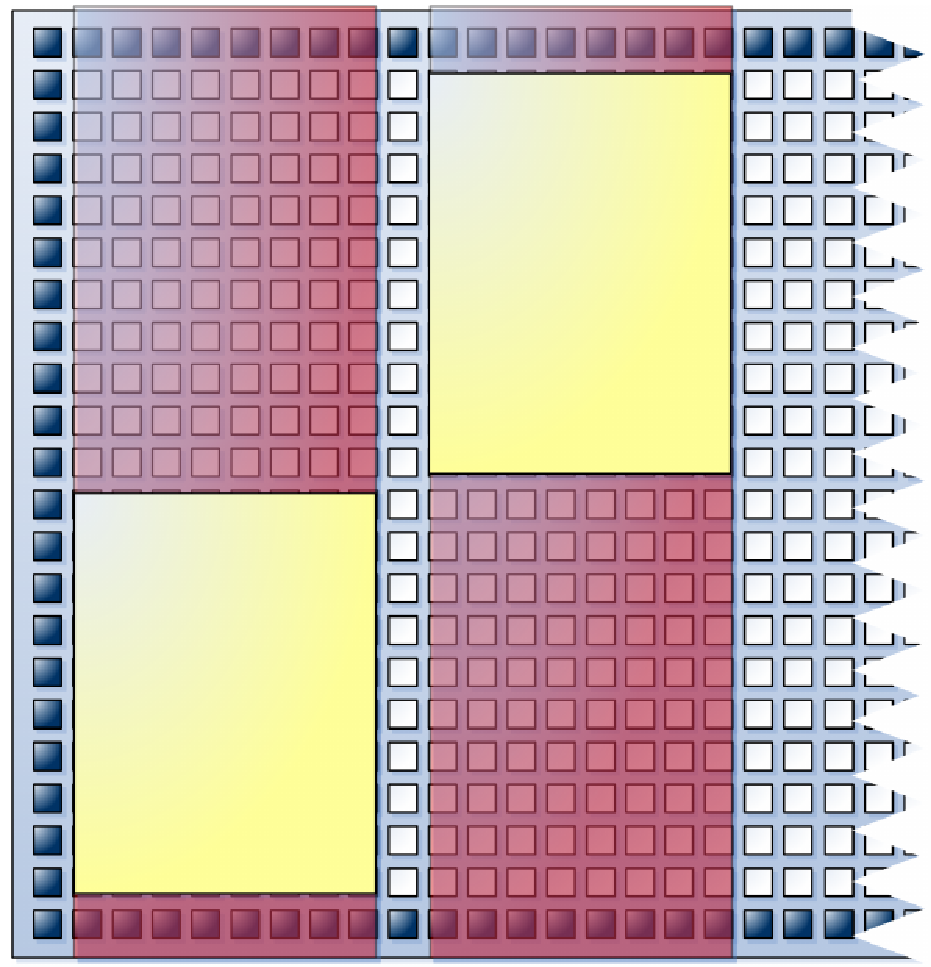
\includegraphics[width=0.7\linewidth]
{capitoli/figure/cap1/Riconfigurazione1D.pdf}}$
  \end{center}
 \end{minipage}
 \hfill
 \begin{minipage}[b]{0.4\textwidth}
 \begin{center}
    $\vcenter{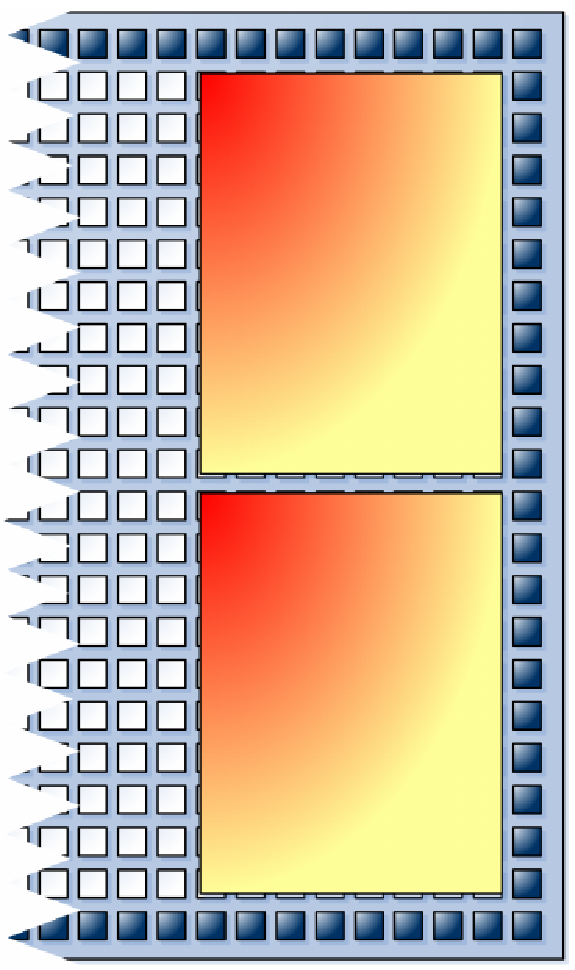
\includegraphics[width=0.45\linewidth]
{capitoli/figure/cap1/Riconfigurazione2D.pdf}}$
 \end{center}
 \end{minipage}
 \caption[Riconfigurazione 1D e 2D]{Riconfigurazione 1D e 2D.\footnotemark}
 \label{fig:riconfigurazione1D2D}
\end{figure}


\subsubsection{Riconfigurazione a due dimensioni}
Le schede \ac{FPGA} moderne riescono a sfruttare, oltre alla riconfigurazione parziale
dinamica, la riconfigurazione bidimensionale, che permette di aumentare il grado di
libertà del designer.

La differenza tra la riconfigurazione a singola dimensione (per colonne) e la
riconfigurazione a due dimensioni è mostrata in figura~\ref{fig:riconfigurazione1D2D}.
Nella riconfigurazione a una dimensione, un modulo che occupa soltanto parte di una
colonna richiede la riconfigurazione di tutta la colonna, il che proibisce il piazzamento
di altri moduli in colonne sovrapposte al primo. La riconfigurazione a due dimensioni
permette, invece, di piazzare i due moduli in un'area della scheda molto più compatta e di
incrementare potenzialmente il numero di moduli che possono essere accelerati se eseguiti
su logica riconfigurabile.

\footnotetext{Immagine tratta da \cite{Redaelli2DILP}.}
L'aumento di versatilità derivante dall'uso della riconfigurazione parziale dinamica
a due dimensioni comporta un notevole sforzo da parte del designer del sistema,
che deve capire quando usare la riconfigurazione permetta un guadagno di prestazioni
e quali moduli riconfigurare, oltre a come piazzare fisicamente questi moduli per sfruttare al
meglio l'area a disposizione.


\section[Alcuni framework di sviluppo per \acs{MPSoC}]{Alcuni framework di sviluppo per \acs{MPSoC}}
\label{sec:flussiLetteratura}
% TODO
